\documentclass[10pt,letterpaper]{article}
\usepackage[T1]{fontenc}
\usepackage[utf8]{inputenc}
\usepackage{lmodern}
\usepackage{microtype}
\usepackage[margin=0.78in,top=0.82in,bottom=0.8in,columnsep=0.27in]{geometry}
\usepackage{amsmath,amssymb,booktabs,array}
\usepackage{graphicx}
\usepackage{tikz}
\usetikzlibrary{arrows.meta,positioning,shapes.geometric}
\usepackage[colorlinks=true,urlcolor=blue!60!black,linkcolor=blue!60!black,citecolor=blue!60!black]{hyperref}
\usepackage{fancyhdr}
\usepackage{enumitem}
\usepackage{xcolor}
\usepackage{multicol}
\usepackage{caption}
\setlist[itemize]{leftmargin=*,nosep,topsep=3pt,parsep=1pt}
\setlength{\parindent}{1em}
\setlength{\parskip}{2.2pt}
\setlength{\columnsep}{0.27in}
\pagestyle{fancy}
\fancyhf{}
\fancyhead[L]{\footnotesize SUPER-GENIUS TECHNICAL MANUSCRIPTS}
\fancyhead[R]{\footnotesize NOVEMBER 2026}
\fancyfoot[C]{\thepage}
\renewcommand{\headrulewidth}{0.35pt}
\newcommand{\figstep}[1]{\tikz[baseline=(X.base)]\node[draw=black!55,rounded corners=2pt,fill=black!3,inner sep=5pt,text width=0.85\columnwidth,align=center,minimum height=0.34in] (X) {\footnotesize #1};}
\newcommand{\sourceline}{\vspace{1pt}\noindent\textit{Scope note:} This manuscript presents an architecture and its analysis. A design description is not an empirical security proof.}

\begin{document}

\begin{center}
{\Large\bfseries Zero-Knowledge Transaction Authentication\\with Append-Only CRDT Credential State\par}
\vspace{7pt}
{\normalsize Kenneth Hurley\par}
\vspace{2pt}
{\small \url{https://super-genius.github.io}\par}
\vspace{4pt}
{\footnotesize Independent technical manuscript \quad | \quad Version 1.0 \quad | \quad November 1, 2026}
\end{center}
\begin{abstract}
Decentralized applications need transaction authentication that remains auditable when account data is replicated among nodes. This manuscript describes an architecture that combines two-factor authentication, encrypted credential storage, a zero-knowledge transaction authorization concept, and an append-only conflict-free replicated data type (CRDT) over content-addressed storage. It outlines credential enrollment, transaction authorization, independent verification, secret rotation, and recovery, then separates the guarantees of each layer. The design aims to preserve transaction integrity while minimizing disclosure of authentication secrets. No working end-to-end proving system, formal convergence proof, or benchmark measurements are asserted.
\end{abstract}
\vspace{3pt}
\noindent\textbf{Keywords:} decentralized authentication; TOTP; CRDT; IPFS; zero-knowledge proofs; audit trail
\vspace{15pt}
\begin{multicols}{2}

\section{Introduction}
Central account systems can authenticate a user and keep an audit record, but the account server can become a single operational failure point. A distributed system must coordinate account enrollment, credential changes, and transaction authorization despite delayed or conflicting updates. It must also protect the secrets used for two-factor authentication (2FA).

This manuscript describes a proposed design built from time-based one-time passwords (TOTP), elliptic-curve-based signatures and encryption, zero-knowledge transaction proofs, and replicated append-only records. The purpose is to separate four concerns: authenticating a user, checking a transaction, storing credential state, and deciding which replicated record is current.

\section{Architecture and Trust Boundaries}
The source divides the system into security initialization, transaction initiation, proof generation, transaction submission, and transaction verification. A distributed account database stores encrypted secret material and an audit trail. Its design refers to IPFS content addressing and CRDT-based replication; the two mechanisms solve different problems.

\begin{center}
\begin{minipage}{\columnwidth}
\centering
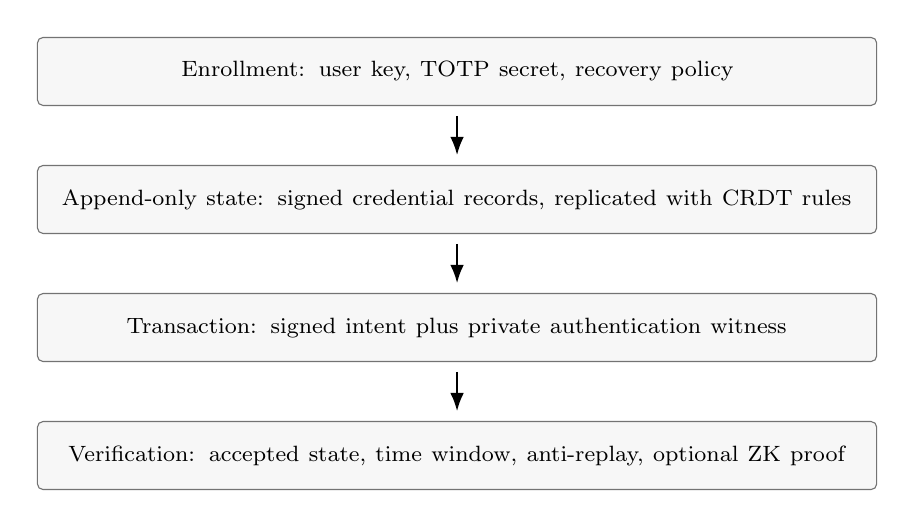
\begin{tikzpicture}[node distance=5mm,>=Latex]
\node (a) {\figstep{Enrollment: user key, TOTP secret, recovery policy}};
\node[below=of a] (b) {\figstep{Append-only state: signed credential records, replicated with CRDT rules}};
\node[below=of b] (c) {\figstep{Transaction: signed intent plus private authentication witness}};
\node[below=of c] (d) {\figstep{Verification: accepted state, time window, anti-replay, optional ZK proof}};
\draw[->,thick] (a.south)--(b.north); \draw[->,thick] (b.south)--(c.north); \draw[->,thick] (c.south)--(d.north);
\end{tikzpicture}
\captionof{figure}{The proposed authentication flow separates replicated state from the proof of a transaction's authority.}
\end{minipage}
\end{center}

CRDTs are designed to merge concurrent updates according to deterministic rules \cite{shapiro}. IPFS provides content-addressed storage and retrieval \cite{ipfs}. Neither one, on its own, makes an account update authorized or an old credential revoked. Signed state transitions, causal ordering, conflict rules, and validation policy are needed.

\section{Credential Enrollment}
During enrollment the system creates or accepts a public-key identity, initializes a TOTP secret, and records how authentication and recovery will work. The source proposes encrypted seed storage and an append-only record of credential creation and changes. Authenticator apps normally receive the original TOTP secret through a QR code or enrollment string; encryption at rest does not remove the need to secure that one-time transfer.

For a time $T$, step size $X$, and initial time $T_0$, TOTP evaluates the HOTP construction on a counter,
\begin{equation}
 C_T=\left\lfloor\frac{T-T_0}{X}\right\rfloor,
\end{equation}
\begin{equation}
 \operatorname{TOTP}_K(T)=\operatorname{Trunc}(\operatorname{HMAC}_K(C_T)).
\end{equation}
Here $K$ is the shared secret and the counter is encoded as specified by the TOTP standard \cite{totp}. The scheme's time dependence requires an explicit acceptance window and a strategy for clock drift.

\section{Transaction Authorization}
The proposed transaction process gathers the intended recipient, amount, and other transaction fields, obtains a second-factor value, and binds the authentication to a transaction signature. The zero-knowledge component seeks to prove that authorization conditions hold without releasing sensitive witness data.

An illustrative proof statement may bind a transaction digest $h(m)$, an accepted credential-state commitment $c$, and a public time interval $t$. A witness can contain secret authentication material and values needed to show that the current credential authorizes the signed intent. The exact relation is part of the protocol design, not something an unspecified zk-SNARK provides automatically.

\begin{equation}
 \operatorname{Verify}(\pi, h(m),c,t)=1.
\end{equation}
A valid proof for this relation should not itself be usable to authorize a different transaction. It should bind to a network identity, request nonce, expiry rule, and transaction fields. A verifier must also check the credential was active at the relevant time and that an earlier proof has not already been consumed where replay is forbidden.

\section{Append-Only Replicated State}
An append-only record can preserve evidence of the history of credential updates. Each transition should carry a monotonically ordered or causally linked identifier, a credential reference, an action such as create/rotate/revoke, and a valid authorization. Replicas may see entries in a different order; they must still agree on which credential is active.

A possible record shape is:
\begin{equation}
 R_i=(\mathrm{id},\mathrm{parent},\mathrm{op},\mathrm{commit},\mathrm{sig}).
\end{equation}
This notation is illustrative. It adds explicit linkage and signatures to show the conditions a secure deployment would need, rather than claiming these fields are present in the source implementation. A signed record can be tamper-evident, but long-term availability still depends on replication, pinning, and storage policy.

\section{Secret Rotation and Recovery}
A secret may be rotated when a device is lost, a key is compromised, or the user changes authenticators. Replication raises a practical question: what happens when two valid-looking changes arrive concurrently? The system needs one deterministic, authorized resolution, with old credentials becoming invalid for new transactions. Merely appending a newer encrypted blob does not establish revocation.

The supplied design discusses server-protected seeds, hardware security modules, backup codes, and recovery through additional authentication channels. These are possible defenses, not interchangeable methods. Recovery channels and any administrator override should be tested as high-value attack targets. Rotating a secret without a valid recovery method cannot recover ciphertext for which all decryption keys are lost.

\section{Threats and Scope}
The principal risks are stolen authentication secrets, stolen signing keys, replayed proofs, malicious state updates, inconsistent replica views, and compromised recovery channels. The protocol must also preserve the independence of the two authentication factors. If both factors can be recovered from the same compromised key or publicly replayable message, the claimed 2FA benefit may disappear.

The use of an append-only CRDT should not be described as a guarantee against modification unless the system verifies signatures, content hashes, and accepted state ancestry. Similarly, zero knowledge protects the hidden witness only for a correctly constructed and verified proof; it does not hide public metadata or repair compromised endpoint security.

\section{Practical Evaluation}
The following tests would define the operational limits of the design, without requiring institutional laboratory infrastructure.

\begin{center}
\begin{minipage}{\columnwidth}
\centering\small
\begin{tabular}{p{0.32\columnwidth}p{0.55\columnwidth}}
\toprule
Scenario & Expected question to answer\\
\midrule
Partition and merge & Do honest replicas agree on active state?\\
Concurrent rotation & Is there one authorized resolution?\\
Replay of proof & Is a reused transaction rejected?\\
Clock skew & Are TOTP windows enforced consistently?\\
Data loss & Can records and encrypted seeds be restored?\\
\bottomrule
\end{tabular}
\captionof{table}{Suggested system tests; no results are claimed here.}
\end{minipage}
\end{center}

\section{Applications and Conclusion}
The architecture can inform distributed wallet logins, token transaction authorization, and access controls for decentralized compute services. Its central design choice is to let peers audit an authorized credential history while verifying a transaction under the current state. The proposed layers are technically compatible, but their joint security depends on clear state-transition rules, a complete proof statement, safe seed handling, and adversarial testing.

\end{multicols}
\vspace{6pt}
\begin{thebibliography}{99}

\bibitem{totp} D. M'Raihi et al., ``TOTP: Time-Based One-Time Password Algorithm,'' RFC 6238, 2011.
\bibitem{hotp} D. M'Raihi et al., ``HOTP: An HMAC-Based One-Time Password Algorithm,'' RFC 4226, 2005.
\bibitem{shapiro} M. Shapiro et al., ``Conflict-free replicated data types,'' in \emph{Symposium on Self-Stabilizing Systems}, 2011.
\bibitem{ipfs} J. Benet, ``IPFS---Content addressed, versioned, P2P file system,'' arXiv:1407.3561, 2014.
\bibitem{zk} E. Ben-Sasson et al., ``Succinct non-interactive zero knowledge for a von Neumann architecture,'' \emph{USENIX Security}, 2014.
\bibitem{source} Author-supplied technical design specification for secure digital transactions, 2024.

\end{thebibliography}
\vspace{6pt}
\noindent\rule{\textwidth}{0.3pt}
\noindent\footnotesize Prepared for publication at \url{https://super-genius.github.io}. This work is a technical exposition, not a claim of independent certification or completed performance evaluation.
\end{document}
